% \todo{Do it.}

% \section{Client Participation}

% \begin{figure}[!ht]
%     \centering
%     \centering
%     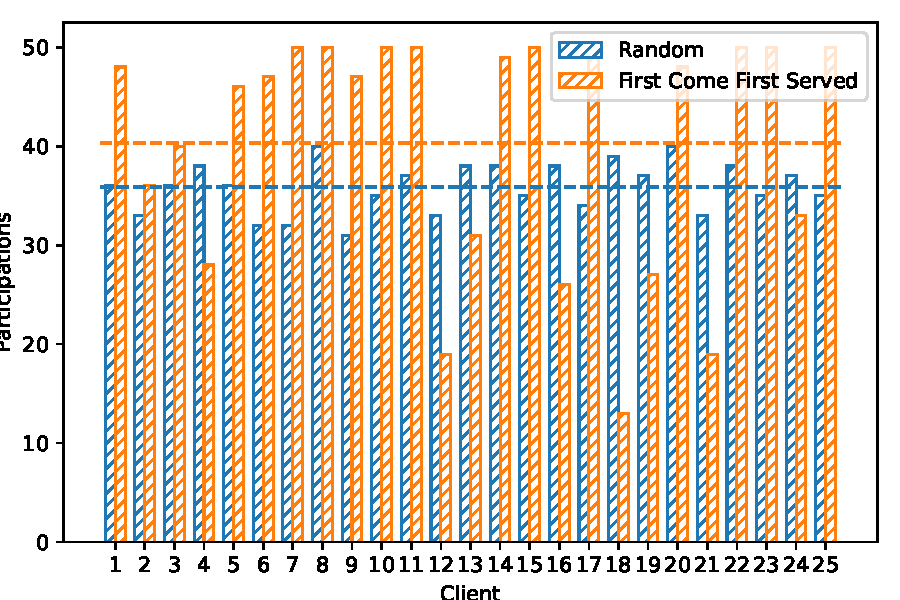
\includegraphics[width=0.7\textwidth]{graphics/02_selection_clients.pdf}
%     \caption{Participation of Each Client Per Selection Technique}
%     \label{fig:participations_client}
% \end{figure}

% \section{Execution Time, Transaction Cost and Latency}

% \begin{table}[!ht]
% \begin{tabular}{c|c|c} \hline \hline
%                               & First Come First Served & Random \\ \hline \hline
% E2E Time (m)                   & 19.70                   & 18.93  \\ \hline
% Mean Round Time (s)            & 23.62                   & 22.70  \\ \hline
% % Median Round Time (s)          & 22.06                   & 21.90  \\ \hline
% Mean Transaction Latency (s)   & 1.560                   & 1.549  \\ \hline
% % Median Transaction Latency (s) & 1.561                   & 1.549  \\ \hline
% Mean Transaction Cost (Gas)    & 189179                  & 183124 \\ \hline
% % Median Transaction Cost (Gas)  & 223471                  & 185198 \\ \hline
% \end{tabular}
% \caption{Time and Transaction Metrics Per Participant Selection Technique}
% \label{tab:metrics_selection}
% \end{table}

\section{Accuracy and Convergence}

\begin{figure}[!ht]
    \centering
    \begin{subfigure}[b]{0.49\textwidth}
        \centering
        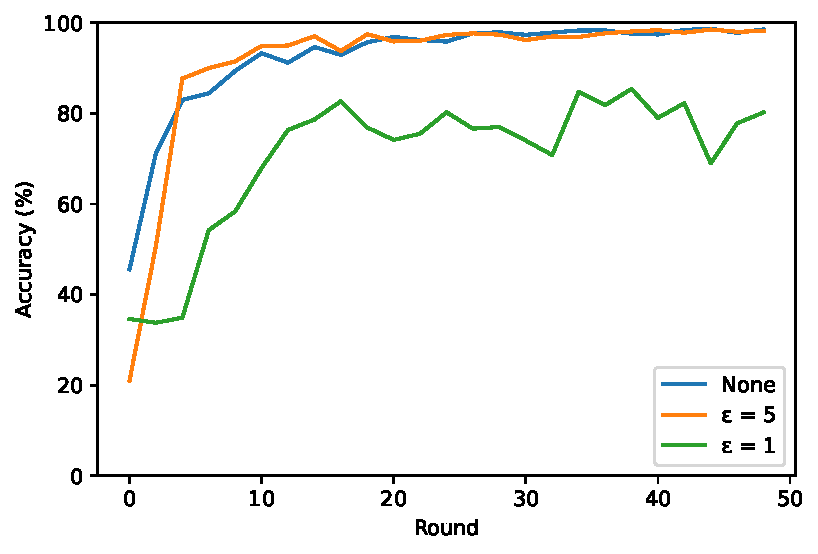
\includegraphics[width=\textwidth]{graphics/05_priv_accuracy_none.pdf}
        \caption{None}
    \end{subfigure}
    \hfill
    \begin{subfigure}[b]{0.49\textwidth}
        \centering
        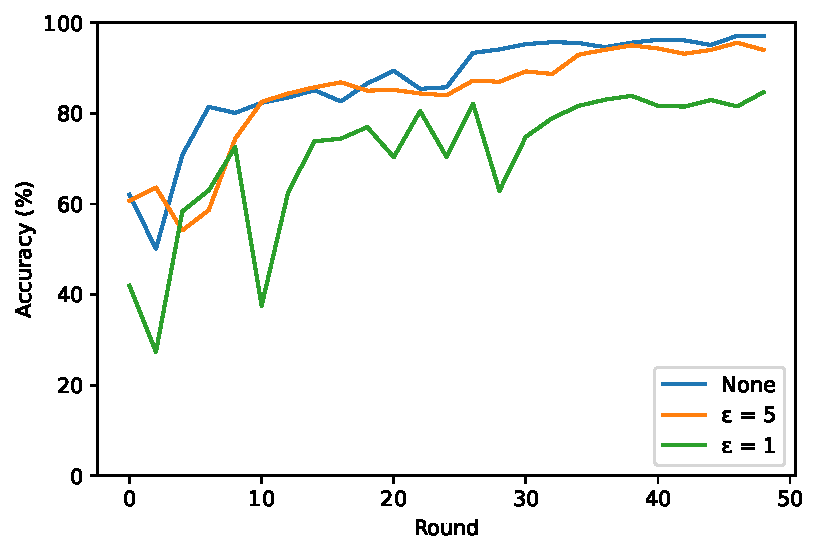
\includegraphics[width=\textwidth]{graphics/05_priv_accuracy_blockflow.pdf}
        \caption{BlockFlow}
    \end{subfigure}
    \hfill
    \begin{subfigure}[b]{0.49\textwidth}
        \centering
        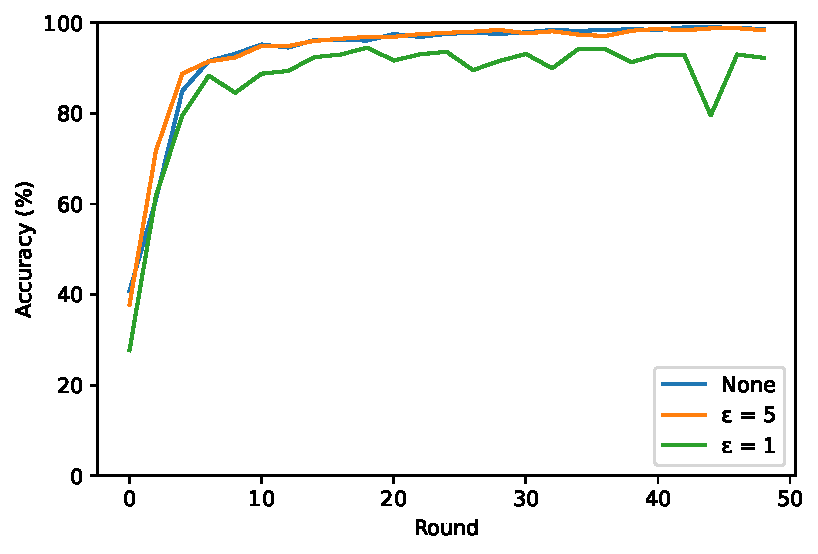
\includegraphics[width=\textwidth]{graphics/05_priv_accuracy_marginalgain.pdf}
        \caption{Marginal Gain}
    \end{subfigure}
    \hfill
    \begin{subfigure}[b]{0.49\textwidth}
        \centering
        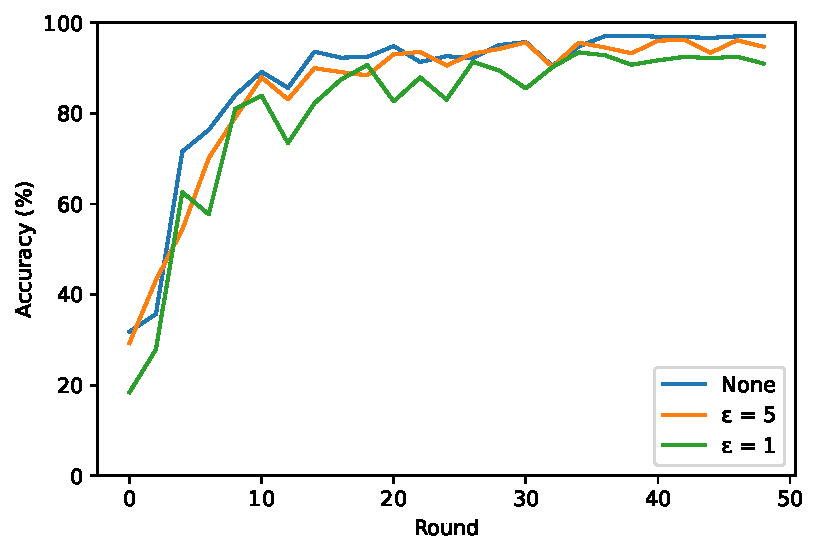
\includegraphics[width=\textwidth]{graphics/05_priv_accuracy_multikrum.pdf}
        \caption{Multi-KRUM}
    \end{subfigure}
    \caption{Accuracy Per LDP Level Per Scoring Technique}
    \label{fig:accuracy_priv}
\end{figure}

% \section{Communication Costs}

% \begin{figure}[!ht]
%     \centering
%     \centering
%     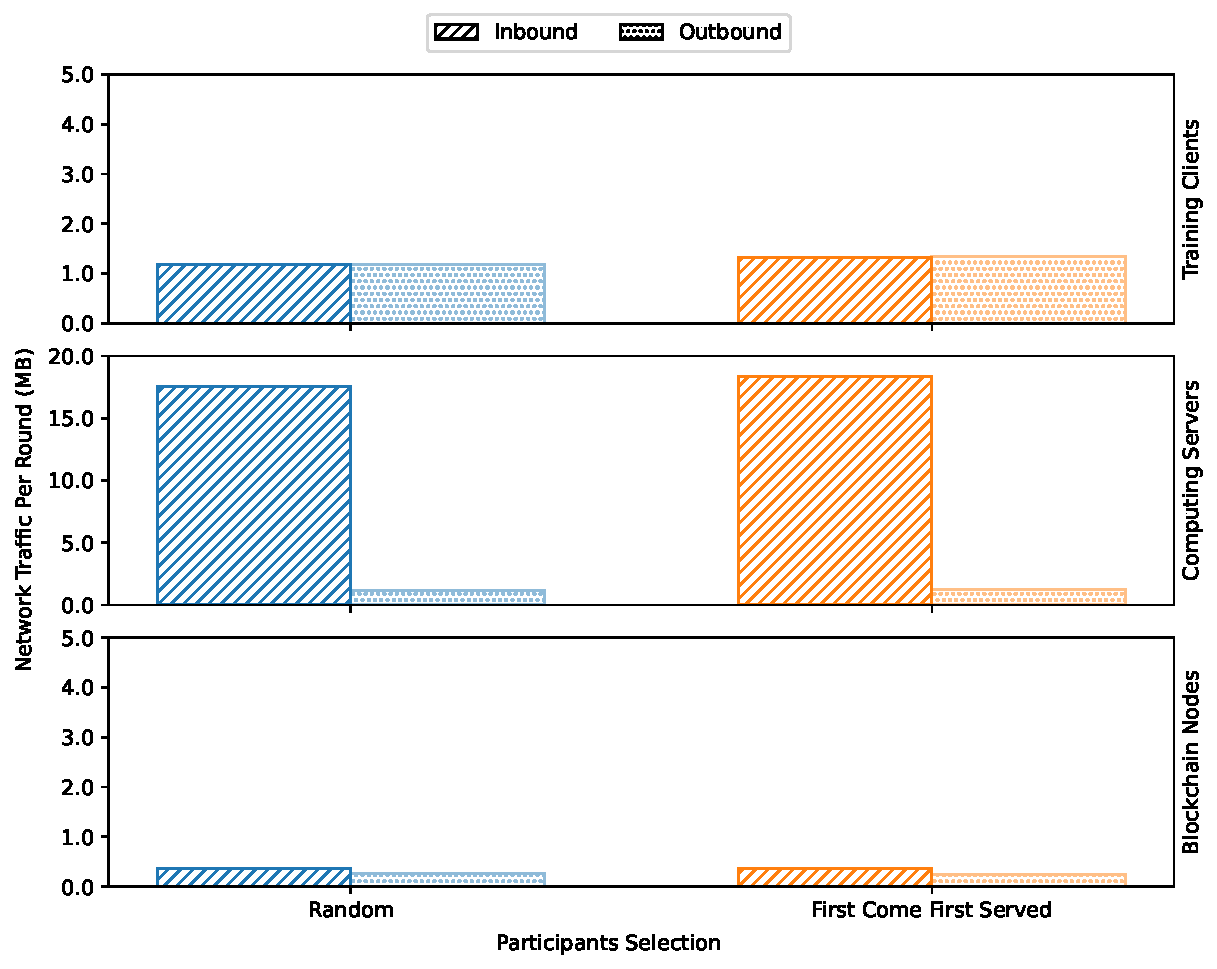
\includegraphics[width=0.8\textwidth]{graphics/02_selection_net.pdf}
%     \caption{Network Traffic Per Round Per Participant Selection technique}
%     \label{fig:net_selection}
% \end{figure}

% \section{Computation Costs}

% \begin{figure}[!hpt]
%     \centering
%     \centering
%     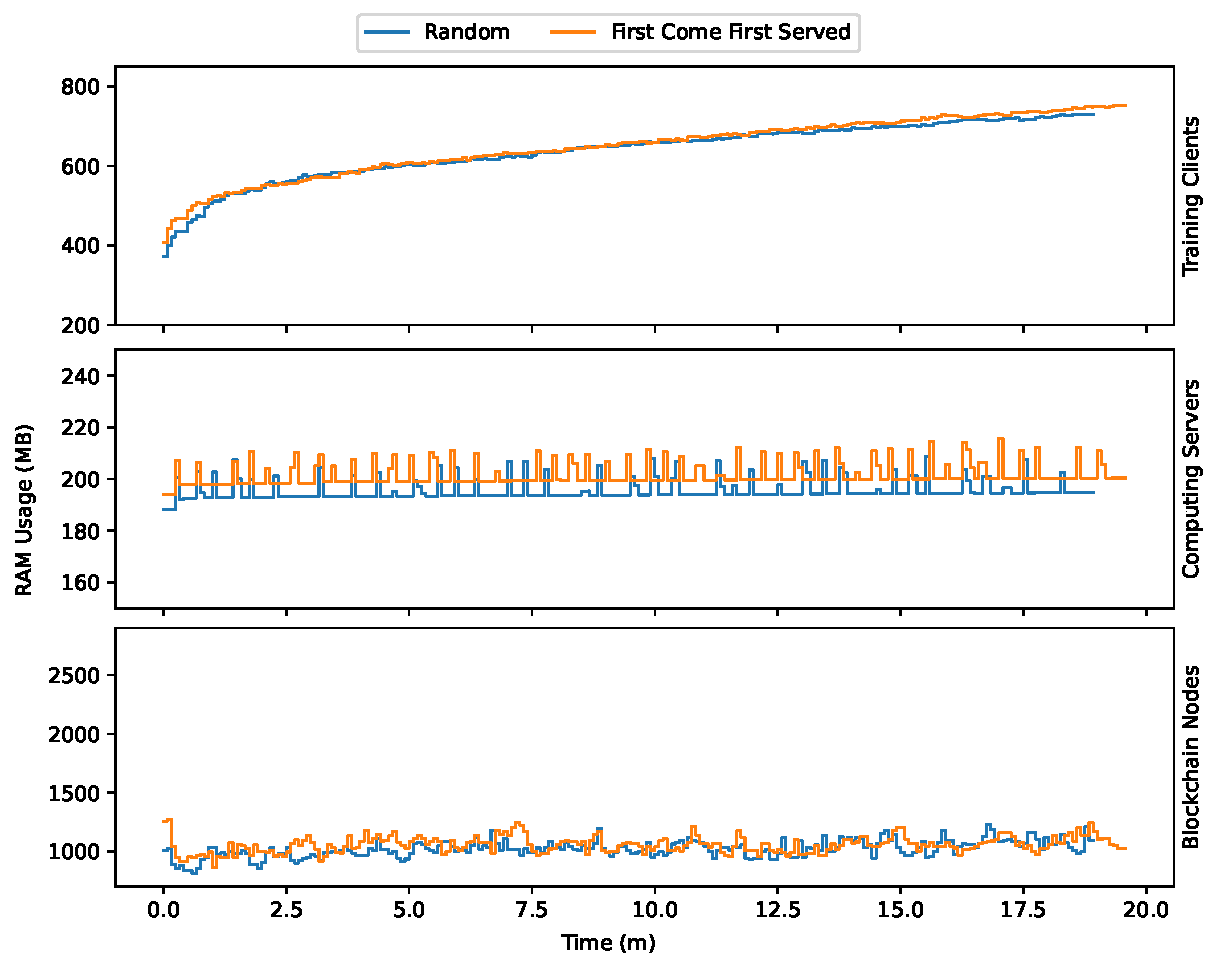
\includegraphics[width=0.8\textwidth]{graphics/02_selection_ram.pdf}
%     \caption{RAM Usage Per Participant Selection technique}
%     \label{fig:ram_selection}
% \end{figure}

% \begin{figure}[!hpb]
%     \centering
%     \centering
%     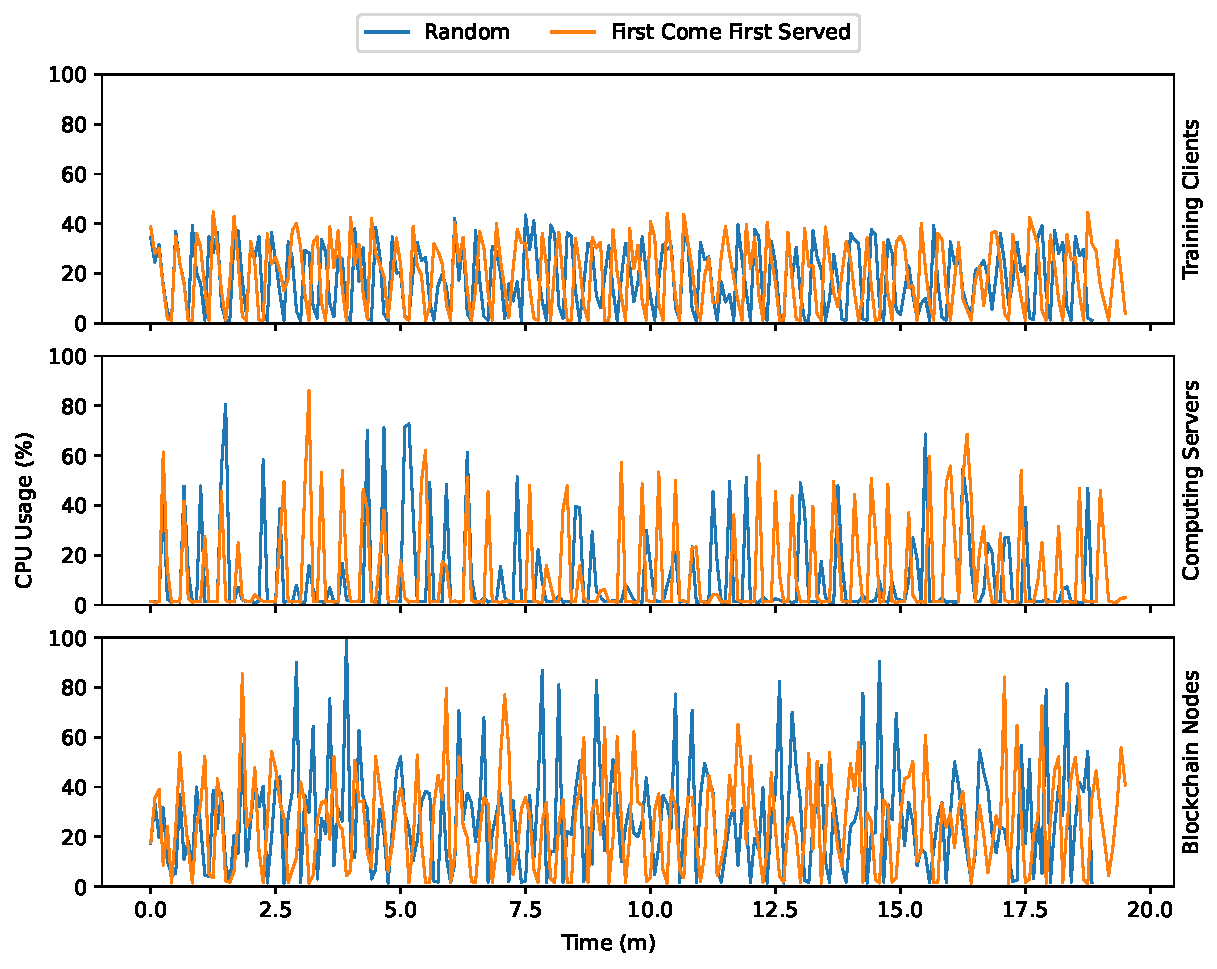
\includegraphics[width=0.8\textwidth]{graphics/02_selection_cpu.pdf}
%     \caption{CPU Usage Per Participant Selection technique}
%     \label{fig:cpu_selection}
% \end{figure}

% \section{Conclusions} % and improvements? and limitations?
